\documentclass[11pt,handout]{beamer}

\usepackage{tcolorbox}
\usepackage{minted}
\usepackage{pdfpages}
\usepackage{sourcecodepro}
\usepackage{graphicx}
\usepackage{amsmath}
\usepackage{fullpage}
\usepackage{bussproofs}
\usepackage{mathpartir}
\usepackage{prooftrees}
\usepackage{color}
\usepackage{algorithmicx}
\usepackage{algpseudocode}

\usetikzlibrary{calc}

\graphicspath{{img/}}

\usetheme{CambridgeUS}
\setbeamertemplate{\insertframenumber/\inserttotalframenumber}

\title[Computer Chess]{Bisimulation Minimization and Symbolic Model Checking}
\author{Sylvain Julmy}
\date{\today}

\begin{document}

\maketitle

\begin{frame}
  \frametitle{LY}
  The Lee-Yannakakis algorithm
\end{frame}

\begin{frame}
  \frametitle{LY - idea}
  \begin{itemize}
  \item Stabilize only reachable blocks.
  \item Reachable block use a representative that has to bee reachable.
  \item The first state is the representative for the initial block.
  \item To find new reachable state, we look for transition from representative
    of reachable state to state from unreachable block.
  \end{itemize}
\end{frame}

\begin{frame}
  \frametitle{LY - idea}
  Two loops :
  \begin{itemize}
  \item Search new reachable blocks
  \item Stabilize reachable but unstable blocks
  \end{itemize}
\end{frame}

\begin{frame}
  \frametitle{LY - termination}
  With the exception of the initial block, all new blocks created by the
  algorithm have paths to the bad block.
\end{frame}

\begin{frame}
  \frametitle{LY - termination}
  Therefore, when a second block becomes reachable, the algorithm should raise a
  violation and terminate.
\end{frame}

\begin{frame}
  \frametitle{LY - new algorithm}
  Basic idea\footnote{Very similar to BR} :
  \begin{itemize}
  \item Search new reachable blocks.
  \item Stabilize reachable but unstable blocks.
  \item When a second block becomes reachable $\to$ raise a violation.
  \end{itemize}
\end{frame}

\begin{frame}
  \frametitle{LY - search}
  To search for new reachable block, the algorithm is searching from all the
  successor of the initial state if one of those is in a different block.

  \pause
  \vspace*{1cm}

  The algorithm also determine if the initial block has to be stabilize or not.
\end{frame}

\begin{frame}[fragile]
  \frametitle{LY - search}
  \begin{algorithmic}
    \State{$D := post(B)$}
    \ForAll{$\langle {C,q} \rangle \in post(init)$}
    \If{$B \neq C$}
    \State{raise violation}
    \EndIf
    \If{$B \cap pre(C) \neq B$} \Comment{Not all predecessor of $B$ are in $B$}
    \State{$B$ is not stable}
    \EndIf
    \State{$D := D - C$}
    \EndFor
    \If{$D \neq \emptyset$} \Comment{$post(init) = \emptyset$}
    \State{$B$ is not stable}
    \EndIf
  \end{algorithmic}
\end{frame}

\begin{frame}[fragile]
  \frametitle{LY - search}
  \begin{columns}
    \begin{column}{0.5\textwidth}
      \begin{align*}
        & queue := \emptyset \\
        & partition = \{B, Bad\} \\
        & init = G_0 \\
        & B = \{G_0,\dots,G_2\}\\
        & Bad = \{B_0,B_1\} \\
        & block_{init} = \langle B,init \rangle \\
        & D = post(B) = \{ B,Bad \}
      \end{align*}
    \end{column}
    \begin{column}{0.5\textwidth}%
      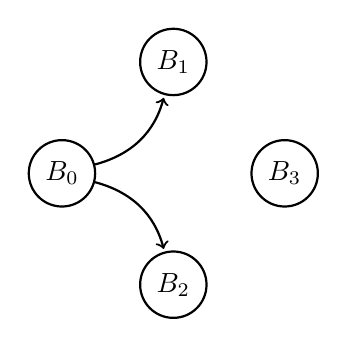
\begin{tikzpicture}[->,shorten >=1pt,auto,node distance=2cm,
                thick,main node/.style={circle,draw,font=\bfseries}]
	\node[main node] (1) {$B_{0}$};
	\node[main node] (2) [above right of = 1] {$B_1$};
	\node[main node] (3) [below right of = 1] {$B_2$};
	\node[main node] (4) [below right of = 2] {$B_3$};

	\path
	(1) edge [bend right] node {} (2)
	(1) edge [bend left] node {} (3)
;
\end{tikzpicture}
    \end{column}
  \end{columns}
\end{frame}
  
\begin{frame}[fragile]
  \frametitle{LY - search}
  \begin{columns}
    \begin{column}{0.5\textwidth}
      \begin{align*}
        & post(init) = \{B\} \\
        & \langle {C,q} \rangle = \langle {B,init} \rangle \\
        & pre(C) = \{ B \} \\
        & \{B\} \cap pre(C) = \{B\} == \{B\} \\
        & D = \{B,Bad\} - \{B\} = Bad \\
        & D \neq \emptyset \to enqueue(\langle {B,init} \rangle)
      \end{align*}
    \end{column}
    \begin{column}{0.5\textwidth}%
      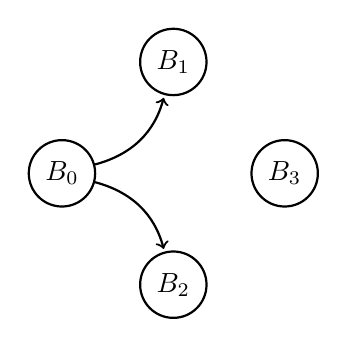
\begin{tikzpicture}[->,shorten >=1pt,auto,node distance=2cm,
                thick,main node/.style={circle,draw,font=\bfseries}]
	\node[main node] (1) {$B_{0}$};
	\node[main node] (2) [above right of = 1] {$B_1$};
	\node[main node] (3) [below right of = 1] {$B_2$};
	\node[main node] (4) [below right of = 2] {$B_3$};

	\path
	(1) edge [bend right] node {} (2)
	(1) edge [bend left] node {} (3)
;
\end{tikzpicture}
    \end{column}
  \end{columns}
\end{frame}

\begin{frame}[fragile]
  \frametitle{LY - stabilization}
  \begin{algorithmic}[1]
    \While{$B$ is not stable}
    \State{Mark $B$ as stable}
    \State{Compute the frontier of $B$}
    \State{Let $B'$ the state of $B$ that can only reach $B$}
    \State{Let $B''$ the state of $B$ that can reach a bad block}
    \If{$\emptyset \neq B' \cap pre(B') \neq B'$ or $\emptyset \neq B' \cap pre(B'')
      \neq B'$}
    \State{Mark $B$ as unstable}
    \EndIf
    \EndWhile
  \end{algorithmic}
\end{frame}

\begin{frame}[fragile]
  \frametitle{LY - stabilization}
  \begin{columns}
    \begin{column}{0.5\textwidth}
      Iteration 1
      \begin{align*}
        & init = G_0 \\
        & partition = \{B,Bad\} \\
        & B = \{G_0,G_1,G_2\} \\
        & pre(B) = \{B\} \\
        & post(B) = \{B,Bad\}
      \end{align*}
    \end{column}
    \begin{column}{0.5\textwidth}%
      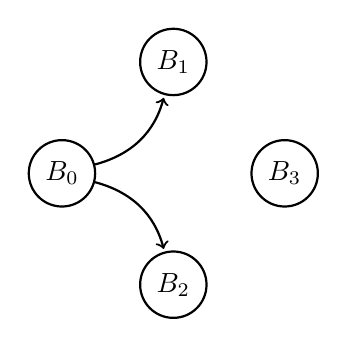
\begin{tikzpicture}[->,shorten >=1pt,auto,node distance=2cm,
                thick,main node/.style={circle,draw,font=\bfseries}]
	\node[main node] (1) {$B_{0}$};
	\node[main node] (2) [above right of = 1] {$B_1$};
	\node[main node] (3) [below right of = 1] {$B_2$};
	\node[main node] (4) [below right of = 2] {$B_3$};

	\path
	(1) edge [bend right] node {} (2)
	(1) edge [bend left] node {} (3)
;
\end{tikzpicture}
    \end{column}
  \end{columns}
\end{frame}

\begin{frame}[fragile]
  \frametitle{LY - stabilization}
  \begin{columns}
    \begin{column}{0.5\textwidth}
      Iteration 1
      \begin{align*}
        & B'_1 = B \cap pre(B) = \{B\} \\
        & B'_2 = pre(post(B) - B) = pre(\{ Bad \}) = \{B\} \\
        & B' = B'_1 - B'_2 = \emptyset \\
        & B'' = B - B' = B \\
        & partition = \{B, Bad, B\} \\
        & B := B' = \emptyset
      \end{align*}
    \end{column}
    \begin{column}{0.5\textwidth}%
      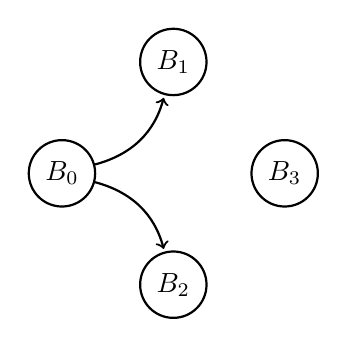
\begin{tikzpicture}[->,shorten >=1pt,auto,node distance=2cm,
                thick,main node/.style={circle,draw,font=\bfseries}]
	\node[main node] (1) {$B_{0}$};
	\node[main node] (2) [above right of = 1] {$B_1$};
	\node[main node] (3) [below right of = 1] {$B_2$};
	\node[main node] (4) [below right of = 2] {$B_3$};

	\path
	(1) edge [bend right] node {} (2)
	(1) edge [bend left] node {} (3)
;
\end{tikzpicture}
    \end{column}
  \end{columns}
\end{frame}

\begin{frame}[fragile]
  \frametitle{LY - stabilization}
  \begin{columns}
    \begin{column}{0.5\textwidth}
      Iteration 1
      \begin{align*}
        & B := B' = \emptyset \\
        & pre(B) = \emptyset \\
        & B'' = B \\
        & pre(B'') = B \\
        & B \cap pre(B) = \emptyset \\
        & B \cap pre(B'') = \emptyset \\
        & \text{no enqueue !} \\
        & post(init) \cap B'' = \{B\} \cap \{B\} = \{B\}\\
        & \to \text{ raise safety violation !}
      \end{align*}
    \end{column}
    \begin{column}{0.5\textwidth}%
      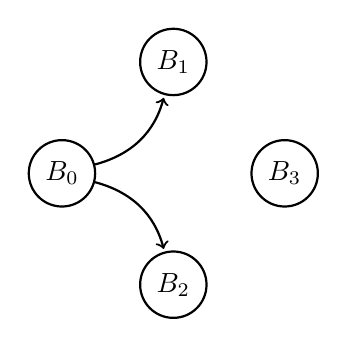
\begin{tikzpicture}[->,shorten >=1pt,auto,node distance=2cm,
                thick,main node/.style={circle,draw,font=\bfseries}]
	\node[main node] (1) {$B_{0}$};
	\node[main node] (2) [above right of = 1] {$B_1$};
	\node[main node] (3) [below right of = 1] {$B_2$};
	\node[main node] (4) [below right of = 2] {$B_3$};

	\path
	(1) edge [bend right] node {} (2)
	(1) edge [bend left] node {} (3)
;
\end{tikzpicture}
    \end{column}
  \end{columns}
\end{frame}

%%%%%%%%%%%%%

\begin{frame}[fragile]
  \frametitle{LY - search (2)}
  \begin{columns}
    \begin{column}{0.5\textwidth}
      \begin{align*}
        & queue := \emptyset \\
        & partition = \{B, Bad\} \\
        & init = G_0 \\
        & B = \{G_0,\dots,G_2\}\\
        & Bad = \{B_0,B_1\} \\
        & block_{init} = \langle B,init \rangle \\
        & D = post(B) = \{ B \}
      \end{align*}
    \end{column}
    \begin{column}{0.5\textwidth}%
      \newcommand*{\con}[2]{(#1) edge [bend left] node {} (#2)}
\begin{tikzpicture}[->,shorten >=1pt,auto,node distance=1.3cm,
                thick,main node/.style={circle,draw,font=\bfseries}]
	\node[main node] (0) {$G_{0}$};
	\node[main node] (1) [below of = 0] {$G_1$};
	\node[main node] (2) [below of = 1] {$G_2$};
	
	\node[main node] (B0) [right of = 0] {$B_{0}$};
	\node[main node] (B1) [below of = B0] {$B_{1}$};
	\path
	\con{0}{1} \con{1}{0}
	\con{1}{2} \con{2}{1}
	\con{B0}{B1}
	(B1) edge [bend left] (2)
;
\end{tikzpicture}
    \end{column}
  \end{columns}
\end{frame}
  
\begin{frame}[fragile]
  \frametitle{LY - search (2)}
  \begin{columns}
    \begin{column}{0.5\textwidth}
      \begin{align*}
        & post(init) = \{B\} \\
        & \langle {C,q} \rangle = \langle {B,init} \rangle \\
        & pre(C) = \{ B , Bad\} \\
        & \{B\} \cap pre(C) = \{B\} == \{B\} \\
        & D = \{B\} - \{B\} = \emptyset \\
        & \text{no safety violation, terminate}
      \end{align*}
    \end{column}
    \begin{column}{0.5\textwidth}%
      \newcommand*{\con}[2]{(#1) edge [bend left] node {} (#2)}
\begin{tikzpicture}[->,shorten >=1pt,auto,node distance=1.3cm,
                thick,main node/.style={circle,draw,font=\bfseries}]
	\node[main node] (0) {$G_{0}$};
	\node[main node] (1) [below of = 0] {$G_1$};
	\node[main node] (2) [below of = 1] {$G_2$};
	
	\node[main node] (B0) [right of = 0] {$B_{0}$};
	\node[main node] (B1) [below of = B0] {$B_{1}$};
	\path
	\con{0}{1} \con{1}{0}
	\con{1}{2} \con{2}{1}
	\con{B0}{B1}
	(B1) edge [bend left] (2)
;
\end{tikzpicture}
    \end{column}
  \end{columns}
\end{frame}

%%%%%%%%%%%%%

\begin{frame}
  \frametitle{LY - complexity}
  \[
    (n-1) * 5M + 4I + 3D + 4E
  \]

  where

  \begin{itemize}
  \item $n$ : number of BR iterations
  \item $M$ : number of image iterations
  \item $I$ : number of intersection operations
  \item $D$ : number of set difference operations
  \item $E$ : number of equality check
  \item $U$ : number of union operations
  \end{itemize}
\end{frame}

\begin{frame}
  \frametitle{BFH}
  The Bouajjani-Fernandez-Halbwachs algorithm
\end{frame}

\begin{frame}
  \frametitle{BFH - idea}
  \begin{itemize}
  \item BFH, like LY, selects reachable blocks to stabilize but differ in how to
    stabilize a block.
  \item BFH stabilize a block w.r.t. all the other blocks (either reachable or
    unreachable).
  \item The algorithm become simplier but unnecessary work is done.
  \end{itemize} 
\end{frame}

\begin{frame}
  \frametitle{BFH - termination}
  As in LY, BFH could terminate when a second block becomes reachable.
  
  The algorithm correctly determine violations of invariants but not as soon as
  they occur.
\end{frame}

\begin{frame}
  \frametitle{BFH - termination}
  The algorthim may traverse a path from the bad block to the initial state
  before the initial block becomes stable.

  Thus, the algorithm take more iteration to terminate.
\end{frame}

\begin{frame}[fragile]
  \frametitle{BFH - new Algorithm}
  \begin{algorithmic}[1]
    \State Mark the bad block
    \State{$I = [init]_p$}
    \While{$I$ is not marked}
    \State{$N := split(I,p)$}
    \If{$N = \{I\}$}
    \State{\textbf{if} $post(I) - I \neq \emptyset$ $\to$ violation, \textbf{else} break}
    \Else
    \State{$p := (p - \{I\}) \cup N$}
    \State{$I := [init]_p$}
    \EndIf
    \EndWhile
    \If{$I$ is marked}
    \State Signal safety violation
    \EndIf
  \end{algorithmic}
\end{frame}

\begin{frame}[fragile]
  \frametitle{BFH - new algorthim (split)}
  \begin{algorithmic}[1]
    \Function{split}{$X$ : block, $p$ : partition}
    \State{$N = \{X\}$}
    \ForAll{$Y$ : block $ \in p$}
    \State{$M := \emptyset$}
    \ForAll{$W$ : state $ \in N$}
    \State{$W_1 = W \cap pre(Y)$}
    \If{$W_1 = W$ or $W_1 = \emptyset$}
    \State{$M := M \cup \{W\}$}
    \Else
    \State{$M := M \cup \{W_1,W - W_1\}$}
    \EndIf
    \EndFor
    \EndFor
    \State{\Return $N$}
    \EndFunction
  \end{algorithmic}
\end{frame}

\begin{frame}
  \frametitle{BFH - example}
  \begin{columns}
    \begin{column}{0.5\textwidth}
      Init
      \begin{align*}
        & I = \{ B \} \\
        & p = \{ B, Bad \} \\
        & init = G_0
      \end{align*}
    \end{column}
    \begin{column}{0.5\textwidth}%
      \input{./tikz/fds_seminar_bfh_a.pgf}
    \end{column}
  \end{columns}
\end{frame}

\begin{frame}
  \frametitle{BFH - example}
  \begin{columns}
    \begin{column}{0.5\textwidth}
      Iteration 1
      \begin{align*}
        & N = split(I,p) = ???
      \end{align*}
    \end{column}
    \begin{column}{0.5\textwidth}%
      \input{./tikz/fds_seminar_bfh_a.pgf}
    \end{column}
  \end{columns}
\end{frame}

\begin{frame}
  \frametitle{BFH - example}
  \begin{columns}
    \begin{column}{0.5\textwidth}
      Iteration 1 - split(1)
      \begin{align*}
        & X = B , p = \{B, Bad\} \\
        & N = \{B\}\\
        & \text{foreach $Y \in p$} \to \\
        & Y = B , M = \emptyset \\
        & \text{foreach $W \in N$} \to \\
        & W = B \\
        & W_1 = W \cap pre(Y) = \{ B \} \\
        & \to M := M \cup \{W\} = \emptyset \cup B = \{B\} \\
        & N := M = \{B\}
      \end{align*}
    \end{column}
    \begin{column}{0.5\textwidth}%
      \input{./tikz/fds_seminar_bfh_a.pgf}
    \end{column}
  \end{columns}
\end{frame}

\begin{frame}
  \frametitle{BFH - example}
  \begin{columns}
    \begin{column}{0.5\textwidth}
      Iteration 1 - split(2)
      \begin{align*}
        & X = B , p = \{B, Bad\} \\
        & N = \{B\}\\
        & \text{foreach $Y \in p$} \to \\
        & Y = Bad , M = \emptyset \\
        & \text{foreach $W \in N$} \to \\
        & W = B \\
        & W_1 = W \cap pre(Y) = B \\
        & Y \text{ is marked} \to B\text{ is marked} \\
        & \to M := M \cup \{W\} = \emptyset \cup \{B\} = \{B\} \\
        & N := M = \{B\} \\
        & return(B)
      \end{align*}
    \end{column}
    \begin{column}{0.5\textwidth}%
      \input{./tikz/fds_seminar_bfh_a.pgf}
    \end{column}
  \end{columns}
\end{frame}

\begin{frame}
  \frametitle{BFH - example}
  \begin{columns}
    \begin{column}{0.5\textwidth}
      Iteration 1
      \begin{align*}
        & N = split(I,p) = \{B\} \\
        & N = \{I\} \to post(I) - \{I\} = \{Bad\} \neq \emptyset \\
        & \to \text{ raise safety violation !}
      \end{align*}
    \end{column}
    \begin{column}{0.5\textwidth}%
      \input{./tikz/fds_seminar_bfh_a.pgf}
    \end{column}
  \end{columns}
\end{frame}

\begin{frame}
  \frametitle{BFH - complexity}
  \[
    (M + I + 2E) * \frac{n^2 + 3n}{2} + n * D
  \]

  where

  \begin{itemize}
  \item $n$ : number of BR iterations
  \item $M$ : number of image iterations
  \item $I$ : number of intersection operations
  \item $D$ : number of set difference operations
  \item $E$ : number of equality check
  \item $U$ : number of union operations
  \end{itemize}
\end{frame}

\begin{frame}
  \frametitle{Experimental comparisons}
  Experimental comparisons
\end{frame}

\begin{frame}
  \frametitle{Experimental comparisons}

  Lower bounds
  
  \begin{itemize}
  \item BR : $n*(M + U + D + 2E + I)$
  \item PT : $n * (2M + D + I + E)$
  \item LY : $(n-1)*(5M + 4I  + 3D + 4E)$
  \item BFH : $(M + I + 2E) * \frac{n^2 + 3n}{2} + n * D$
  \end{itemize}
\end{frame}

\begin{frame}
  \frametitle{Experimental comparisons}
  \begin{itemize}
  \item BR has better time and memory usage (in almost all cases).
  \item PT does surprisingly well w.r.t. LY and BFH
  \end{itemize}
\end{frame}

\begin{frame}
  \frametitle{Experimental comparisons}
  ``That PT performs so well compared to BFH and LY suggests that minimization
  algorithms tailored to verification settings should pay attention ti choosing ''
\end{frame}

\begin{frame}
  \frametitle{Conclusion}
  Bisimulation and Model Checking requires more resources than model checking
  alone.
\end{frame}

\end{document}